
% !TEX encoding = UTF-8 Unicode 
% !TEX root = FieldGuide.tex

\subpart{Two shape parameters}

\Sec{Unit Gamma Distribution} 
\label{sec:UnitGamma}
\dist{Unit gamma} (log-gamma) distribution~\cite{Olshen1938,Consul1971,Grassia1977,Gupta2004}:
% log-gamma\sscite{Consul1971}
\begin{align}
\label{UnitGamma}
\opr{UnitGamma}&(x\given a, s,\alpha,\beta) \\ \notag &= \frac{1}{\Gamma(\alpha)} \Left|\frac{\beta}{ s}\Right|
\Left(\frac{x-a}{s}\Right)^{\beta-1} \Left(-\beta \ln   \frac{x-a}{s} \Right)^{\alpha-1}  \checked
\notag
\\ \text{for }& x,\ a,\ s,\ \alpha,\ \beta \text{ in } \mathbb{R},\ \ \alpha >0
\notag
 \\ \text{ support } & x \in [a,a+s], s>0,\ \beta>0 \notag \\ \text{ or } &  x\in[a+s,a], s<0,\ \beta>0 
 \notag 
 \\  \notag  \text{ or } &  x\in[a+s,+\infty], s>0,\ \beta<0 
 \\  \notag  \text{ or } &  x\in[-\infty,a+s], s<0,\ \beta<0 
\end{align}

A curious distribution that occurs as a limit of the generalized beta \eqref{GenBeta}, and as the anti-log transform of the gamma distribution \eqref{Gamma}. For this reason, it is also sometimes called the log-gamma distribution.

% Note Olsehn1938 uses parameterization with negative of beta used here.}


\SSec{Special cases}


\dist{Uniform product} distribution~\cite{Springer1979a}:
\begin{align}
\label{UniformProduct}
\opr{UniformProduct}(x\given n) &=  \frac{1}{\Gamma(n)} \Left( -\ln x \Right)^{n-1} 	\checked
 \\ \notag & = \opr{UnitGamma}(x\given 0, 1,n,1)							\checked
 \\ \notag & \qquad 0>x>1, \quad n = 1,\ 2,\ 3,\ \ldots							\checked
\end{align}
The product of $n$ standard uniform distributions \eqref{StdUniform}.



\SSec{Interrelations}
With  $\alpha=1$ we obtain the power function distribution \eqref{PowerFn} as a special case.
\[
\opr{UnitGamma}(x\given a, s,1,\beta) = \opr{PowerFn}(x\given a,s,\beta) \checked \notag
\]

The  unit gamma is the anti-log transform of the standard gamma distribution \eqref{StdGamma}.
\begin{align*}
\opr{UnitGamma}(0,1,\alpha,\beta)& \sim \exp\bigl(-\opr{Gamma}(0, \tfrac{1}{\beta}, \alpha)\bigr) \checked
\\
\opr{UnitGamma}(0,1,\alpha,1) &\sim \exp\bigl(-\opr{StdGamma}( \alpha)\bigr) \checked
\end{align*}




The unit gamma distribution is a limit of the generalized beta distribution \eqref{GenBeta}, and limits to the gamma \eqref{Gamma} and log-normal  \eqref{LogNormal}~\cite{\self} distributions.
\[
\opr{Gamma}(x\given a,s,\alpha) &= \lim_{\beta\rightarrow\infty} \opr{UnitGamma}(x\given a+\beta s,-\beta s, \alpha,\beta)
\checked
\notag
\]
\begin{align*}
\lim_{\alpha\rightarrow\infty}& \opr{UnitGamma} (x\given a, \vartheta e^{ \sigma\sqrt{\alpha}}, \alpha, \tfrac{\sqrt{\alpha}}{\sigma})
\checked
\\ 
& \propto  \lim_{\alpha\rightarrow\infty}  \Left(\frac{x-a}{ \vartheta e^{ \sigma\sqrt{\alpha}} }\Right)^{ \tfrac{\sqrt{\alpha}}{\sigma} -1}
\Left(-  \frac{\sqrt{\alpha}}{\sigma} \ln  \frac{x-a}{ \vartheta e^{ \sigma\sqrt{\alpha}} } \Right)^{\alpha-1}
\checked
\\ 
& \propto  \Left(\frac{x-a}{\vartheta}\Right)^{-1}   \lim_{\alpha\rightarrow\infty}
\exp\Left\{\sqrt{\alpha}\frac{1}{\sigma} \ln \frac{x-a}{ \vartheta}\Right\}
\Left( 1 - \frac{1}{\sqrt{\alpha}} \frac{1}{\sigma} \ln  \frac{x-a}{ \vartheta  } \Right)^{\alpha-1}
\checked
\\
& \propto  \Left(\frac{x-a}{\vartheta}\Right)^{-1}   \lim_{\alpha\rightarrow\infty} e^{-z \sqrt{\alpha}}  \bigl( 1+\frac{z}{\sqrt{\alpha}} \bigr)^{\alpha} , \quad  z = -\tfrac{1}{\sigma} \ln \tfrac{x-a}{\vartheta}
\checked
\\
&  \propto \Left(\frac{x-a}{\vartheta}\Right)^{-1} \exp\Left\{-\frac{1}{2\sigma^2} \Left( \ln \frac{x-a}{\vartheta} \Right)^2 \Right\}
\checked
\\
& \quad  =  \opr{LogNormal} (x\given a, \vartheta, \sigma)
\checked
\end{align*}
\label{UnitGammaToLogNormal}
Here we utilize the Gaussian function limit $
\lim_{c \rightarrow \infty} e^{-z \sqrt{c}}  \bigl( 1+\frac{z}{\sqrt{c}} \bigr)^c = e^{-\half z^2} \checked$ \secref{sec:Limits}.
\index{Gaussian function limit}



\begin{figure}[t]
\begin{center}
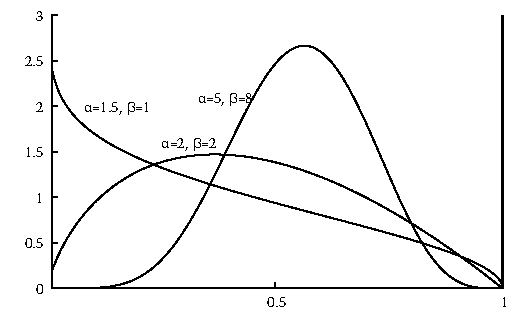
\includegraphics[width=\textwidth]{pdfUnitGamma}
\end{center}
\caption[Unit gamma, finite support.]{Unit gamma, finite support, $\opr{UnitGamma}(x\given 0, 1,\alpha,\beta)$, $\beta>0$.}
\end{figure}

\begin{figure}[t]
\begin{center}
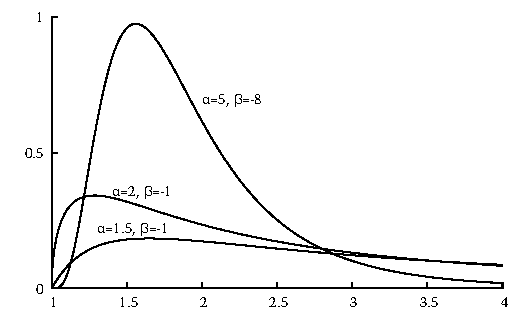
\includegraphics[width=\textwidth]{pdfUnitGammaNegBeta}
\end{center}
\caption[Unit gamma, semi-infinite support.]{Unit gamma, semi-infinite support. $\opr{UnitGamma}(x\given 0, 1,\alpha,\beta)$, $\beta<0$}
\end{figure}



The product of two unit-gamma distributions with common $\beta$ is again a unit-gamma distribution~\cite{Consul1971,\self}. 
\begin{align*}
\opr{UnitGamma}_1 (0,s_1,\alpha_1, \beta )\ & \opr{UnitGamma}_2(0,s_2, \alpha_2, \beta ) 
 \\
&\sim \opr{UnitGamma}_3(0,s_1 s_2,\alpha_1 + \alpha_2, \beta )  \checked
\end{align*}
The property is related to the  analogous additive relation of the gamma distribution.
\begin{align*}
&\opr{UnitGamma}_1(0,s_1,\alpha_1, \beta )\ \opr{UnitGamma}_2(0,s_2, \alpha_2, \beta ) 
\\
&\sim s_1 s_2 \Left(\opr{UnitGamma}_1(0,1,\alpha_1,1)\ \opr{UnitGamma}_2(0,1,\alpha_2,1)  \Right)^{\tfrac{1}{\beta}}
\\
&\sim s_1 s_2 \Left(e^{- \opr{StdGamma}_1(\alpha_1) - \opr{StdGamma}_2(\alpha_2 ) } \Right)^{ \tfrac{1}{\beta}}
\\
&\sim s_1 s_2 \Left(e^{- \opr{StdGamma}_3(\alpha_1+ \alpha_2 )  }\Right)^{\tfrac{1}{\beta}}
\\
&\sim \opr{UnitGamma}_3(0,s_1 s_2,\alpha_1 + \alpha_2, \beta ) \checked
\end{align*}



% !TEX encoding = UTF-8 Unicode 
% !TEX root = FieldGuide.tex

\begin{table*}[t!]
\caption[Unit gamma distribution -- Properties]{Properties of the unit gamma distribution}
\begin{align*}
\text{\hyperref[PropertiesSec]{Properties}}  \quad& \\
\text{notation} \quad & \text{UnitGamma}(x\given a,s,\alpha,\beta) 
\\
\text{PDF}\quad &  \frac{1}{\Gamma(\alpha)} \left|\frac{\beta}{ s}\right|
\left(\frac{x-a}{s}\right)^{\beta-1} \left(-\beta \ln   \frac{x-a}{s} \right)^{\alpha-1} \checked
\\
\text{CDF} \big/ \text{CCDF}  \quad  & 1-Q\left(\alpha, -\beta \ln \tfrac{x-a}{s} \right)
& \tfrac{\beta}{s}  >0 \ \big{/} \ \tfrac{\beta}{s}<0   \checked
\\
\text{parameters}\quad &   a, s,\alpha,\beta \text{ in } \Real  ,\  \alpha, \beta>0
\\
\text{support}\checked \quad 
	&   [a,a+s] ,\ s>0,\ \beta>0 \\
	&  [a+s,a], \ s<0,\ \beta>0 \\
	& [a+s,+\infty]  s>0,\ \beta<0  \\
 	& [-\infty,a+s], s<0,\ \beta<0 \\
%\text{median} \quad  &  \cdots
%\\
%\text{mode} \quad  & a+s \exp \left(\tfrac{1-\alpha}{1-\beta} \right)  \text{ if } \alpha,\beta>0 \text{ or } \alpha,\beta<0 \text{ (antimode)} \hspace{-4em}
%  ????
\\
\text{mean} \quad  &  a + s \left(\tfrac{\beta}{\beta+1} \right)^{\alpha} \checked
\\
\text{variance} \quad  & s^2 \left(\tfrac{\beta}{\beta+2} \right)^{\alpha} - s^2 \left(\tfrac{\beta}{\beta+1} \right)^{2\alpha} \checked
\\
\text{skew} \quad  &   \text{not simple}
\\
\text{kurtosis} \quad  &   \text{not simple}
\\
\text{entropy} \quad  & \cdots
\\
\text{MGF} \quad  &  \cdots
\\
\text{CF} \quad  &  \cdots
\\
E(X^h) \quad & \left(\tfrac{\beta}{\beta+h} \right)^{\alpha} \qquad  & a=0 \
\text{\cite{Grassia1977}} \checked
\end{align*}
\end{table*}

